\chapter{Related Work} \label{chap:Chapter2}       
\epigraph{``This is where technology is now, imagine where we can go in the future” }{\textit{Timothy Chung}}

Σε αυτό το \emph{Chapter} περιγράφονται τρόποι - από την βιβλιογραφία - με τους οποί\-ους, υπάρχουσες εφαρμογές 
μεμονωμένων \hyperref[abbr:UAV]{UAV}, καθώς και drone swarms επιλύουν το localization pro\-blem. Κάποια από τα συστήματα στις παρακάτω έρευνες έχουν καθαρά
θεωρητική πλευρά, ενώ, άλλα έχουν δοκιμαστεί σε real-life scenarios.
Τέλος, σε α\-ρκε\-τές από αυτές τις εφαρμογές χρησιμοποιούνται τεχνικές που θα αναλυθούν στο \emph{Chapter} \ref{chap:Chapter3} 
σε μεγαλύτερο βάθος, καθώς θα αποτελέσουν το προαπαιτούμενο θεωρητικό και μαθηματικό υπόβαθρο για τον σχεδιασμό του συστήματος της παρούσας διπλωματικής.

% Κυρίως, αυτά που θα μελετήσουμε θα αφορούν Cooperative Localization (\hyperref[abbr:CL]{CL}) των \hyperref[abbr:UAV]{UAV}s, ενώ επίσης
% μας ενδιαφέρουν τα Distributed Computation - Real Time Location System (\hyperref[abbr:RTLS]{RTLS}) \cite{rtls}. 

Το πρόβλημα του Local Positioning System 
(\hyperref[abbr:LPS]{LPS}) \cite{lps} έχει ερευνηθεί από διάφορες οπτικές\udot οι οποίες μπορεί να βασίζονται σε Radio Frequency
(\hyperref[abbr:RF]{RF}), Sound Waves ή ακόμα και να είναι Image Oriented.

Σχεδόν βέβαιο είναι επίσης, ότι από όποια κατεύθυνση και αν προσεγγίσουμε το \hyperref[abbr:LPS]{LPS} να έχουμε την ανάγκη να 
χρησιμοποιήσουμε κάποια τεχνική για να συνενώσουμε όλες τις πληροφορίες που έχουμε από τους διάφορους αισθητήρες για κάθε μεμονωμένο 
time-frame - με δεδομένο ότι κάνουμε χρήση πολλαπλών αισθητήρων ώστε να μειώσουμε την εντροπία, συνεπώς και την αβεβαιότητα ως 
προς την εκτίμηση της θέσης. 
Την ανάγκη αυτού έρχεται να καλύψει η έννοια του \emph{sensor fusion} \cite{sensor-fusion}. Όπως επίσης,  
και την ανάγκη φιλτραρίσματος των μετρήσεων - που οδηγεί σε καλύτερα αποτε\-λέ\-σμα\-τα - με μερικούς γνωστούς 
αλγόριθμους που να το επιτυγχάνουν - να είναι το  
Extended Kalman Filter (\hyperref[abbr:EKF]{EKF}), Unscented Kalman Filter (\hyperref[abbr:UKF]{UKF}), Covariance Intersection  
Filter (\hyperref[abbr:CIF]{CIF}),  Split  Covariance  Intersection  Filter (\hyperref[abbr:SCIF]{SCIF}) και  Belief  Propagation 
(\hyperref[abbr:BP]{BP}) \cite{fusion-filters}. 

% Τέλος, είναι επίσης σημαντικό να αναφερθούν τα βασικά \emph{coordinate frames} τα οποία χρησιμοποιούνται. 
% Αισθητήρες όπως το \hyperref[abbr:IMU]{IMU} και το compass κάνουνε μετρήσεις με γνώμονα το ίδιο το σώμα 
% του αντικειμένου για αυτό - σε αυτήν την περίπτωση το σύστημα αξόνων ονομάζεται body frame (B frame) \cite{uwb-imu-gps1}.
% Συχνά είναι όμως βολικό να μετατρέψουμε αυτές τις μετρήσεις σε ένα κοινό North East Down (\hyperref[abbr:NED]{NED}) 
% σύστημα, οπότε τότε αναφερόμαστε σε N frame \cite{uwb-imu-gps1} \cite{body-frames}. Παράδειγμα μεταξύ των δύο 
% συστημάτων βρίσκεται στο \emph{Figure} \ref{fig:Important-coordinate-frames}.

% \begin{figure} [H]
% 	\centering
% 	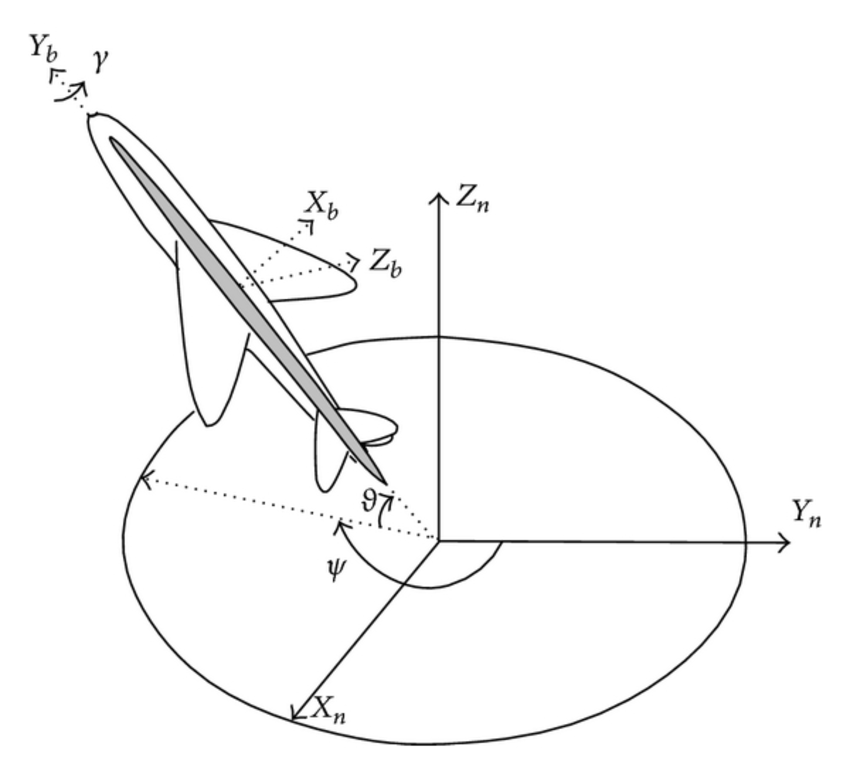
\includegraphics[width=0.6\linewidth]{Images/Related-Work/b-frame-n-frame-and-Euler-angles.png}
% 	\decoRule
% 	\caption[Important coordinate frames]{Important coordinate frames \cite{body-frames}}
% 	\label{fig:Important-coordinate-frames}
% \end{figure}


% ------------------------------------------------------------------------------------
\section{Radio Frequency}
Το πιο εύκολο που μπορούμε να φανταστούμε είναι να χρησιμοποιήσουμε \hyperref[abbr:RF]{RF} τε\-χνο\-λο\-γίες
όπως WiFi, Zigbee και Ultra-Wideband (\hyperref[abbr:UWB]{UWB}) για την επικοινωνία και την υλοποίηση του \hyperref[abbr:LPS]{LPS}.   
Το WiFi είναι εύκολα προσβάσιμο\udot με μικρό κόστος ενώ το Zigbee προτιμάται για
low power consumption εφαρμογές. Όμως προβλήματα αυτών των δύο, μπορεί να είναι, ότι το 
WiFi έχει μικρή εμβέλεια\footnote{Αυτό μπορεί να είναι αρνητικό για κάποιες εφαρμογές σε outdoor scenarios} όπως επίσης είναι πολύ εύκολο 
να υπάρχουν παρεμβολές από τις υπόλοιπες γειτονικές συσκευές\footnote{Αυτό μπορεί να είναι αρνητικό για κάποιες εφαρμογές σε indoor scenarios} 
άρα δεν το καθιστά καλή λύση για κάθε αποστολή ενός swarm. Το Zigbee επιλύει κάποια από αυτά τα 
προβλήματα\footnote{Σε indoor σενάρια παραμένει η δυσκολία για collision-free formation}. Συχνή εφαρμογή έχουν επίσης 
τα \hyperref[abbr:UWB]{UWB} καθώς επιλύει θέματα σχετικά με την ακρίβεια των μετρήσεων, το κόστος καθώς και την 
εμβέλεια\udot ταυτόχρονα \cite{uwb-imu-gps3}. Τέλος, θετικό στην χρήση \hyperref[abbr:RF]{RF} τεχνολογιών, είναι ότι μπορούμε εύκολα να δημιουργήσουμε
ένα Flying Ad-hoc Network (\hyperref[abbr:FANET]{FANET}) το οποίο βοηθάει στην ευελιξία του συστήματος.

 
% ---------------------
\subsection{WiFi}
Μία αρχική προσέγγιση για τον εντοπισμό ενός drone δίνεται από τους συγγραφείς του \cite{wifi-passive-active-drone-localization}
οι οποίοι χρησιμοποιούν WiFi προκειμένου να εντοπίσουν την θέση του αεροχήματος. Το ενδιαφέρον - με την χρήση του WiFi - είναι ότι, 
είναι μία εύκολη λύση όταν αναφερόμαστε για short range localization. 

Ο τρόπος με τον οποίο προσεγγίζουν το πρόβλημα, είναι με 
το να προσπαθήσουν να αξιοποιήσουν - από την πλευρά του WiFi based - τις τεχνικές, 
Passive Bistatic Radar (\hyperref[abbr:PBR]{PBR}) και Passive Source Location (\hyperref[abbr:PSL]{PSL}), να χρησιμοποιήσουν Kalman Filter (\hyperref[abbr:KF]{KF})
και τέλος να πραγματοποιήσουν Data Fusion τεχνικές στους δύο αισθητήρες που χρησιμοποιήθηκαν\udot ώστε να γίνει ο εντοπισμός της θέσης.

Ξεκινώντας με τη τεχνική \hyperref[abbr:PBR]{PBR}, η οποία αξιοποιεί τα echoes που
γίνονται scatter από τα εμπόδια που υπάρχουν στον χώρο\udot προκειμένου να εντοπίσει το αντικείμενο. Έχει σαν κύρια χαρακτηριστικά 
ότι χρησιμοποιείται για εντοπισμό κινούμενων αντικειμένων και δεν χρειάζεται το ίδιο το αντικείμενο να εκπέμπει σήματα, πράγμα που το καθιστά ιδανικό για εντοπισμό 
non-cooperative στόχων. Προκειμένου βέβαια να εκτιμηθεί η θέση, έπειτα από την αρχική επεξεργασία που γίνεται από τα λαμβανόμενα echoes, ο εντοπισμός τελικά της θέσης
πραγματοποιείται μέσω ενός συνδυασμού από μετρήσεις με βάση range είτε γωνία. 

Αντίθετα, με την τεχνική \hyperref[abbr:PSL]{PSL} - η οποία προαπαιτεί stationary αντικείμενα - είναι σημαντικό να λαμβάνουμε πακέτα από το αντικείμενο ενδιαφέροντος,
καθώς εκτιμάει την θέση του\udot μέσω των πακέτων που λαμβάνει, σε συνδυασμό με μία μέτρηση \hyperref[abbr:AoA]{AoA} και μία \hyperref[abbr:TDoA]{TDoA}
(στο \Sect{sec:Energy-based} γίνεται ανάλυση τους).

Συνοπτικά οι συγγραφείς της συγκεκριμένης έρευνας, παρουσιάζουν στο \Fig{fig:PBR-and-PSL} (a) τον γενικό τρόπο λειτουργίας των δύο μεθόδων, ενώ στο
\Fig{fig:PBR-and-PSL} (b) τις διαφορές τους.

\begin{figure} [H]
	\centering
    % -----------------
		\begin{minipage}{.48\textwidth}
			\centering
			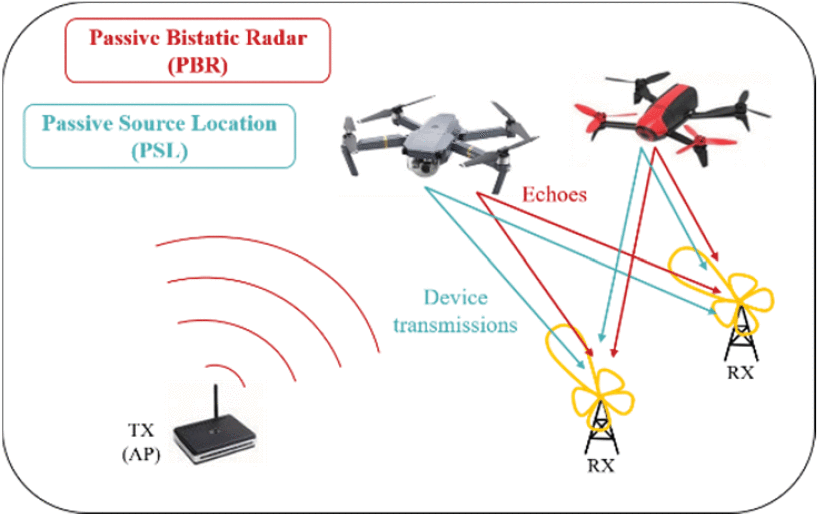
\includegraphics[width=\linewidth]{Images/Related-Work/PBR-and-PSL-approaches.png}
			{(a) PBR and PSL (\href{https://ieeexplore.ieee.org/document/9253794/figures#figures}{URL})}
		\end{minipage}%
		\hspace*{+1cm}
		% -----------------
		\begin{minipage}{.48\textwidth}
			\centering
			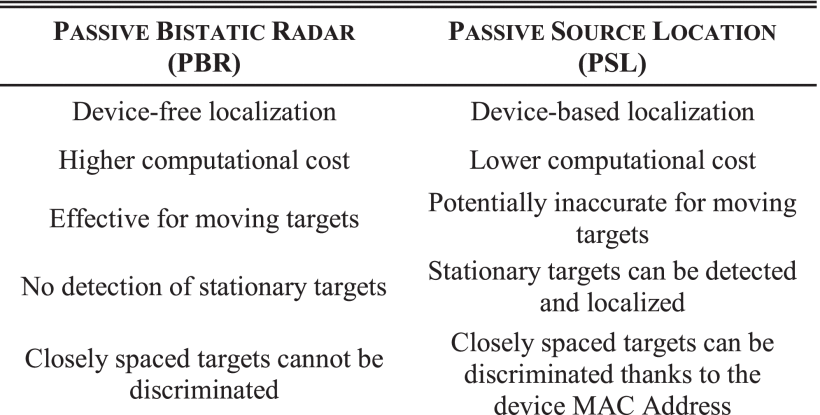
\includegraphics[width=\linewidth]{Images/Related-Work/PBR-and-PSL-Features.png}
			{(b) PBR and PSL Features (\href{https://ieeexplore.ieee.org/document/9253794/figures#figures}{URL})}
		\end{minipage}
	% -----------------
    \hfill \break
    \decoRule
    \caption[PBR and PSL localization Approaches]{PBR and PSL localization Approaches based on \cite{wifi-passive-active-drone-localization}}
    \label{fig:PBR-and-PSL}
\end{figure}

Για την υλοποίηση χρησιμοποιήθηκε ένα DJI Mavic Pro, το οποίο ήταν το drone του οποίου η θέση έγινε προσπάθεια να εκτιμηθεί.
Σχετικά με το σκέλος του \hyperref[abbr:PBR]{PBR} χρησιμοποιήθηκε ένα Access Point (AP, D-Link DAP1160), το οποίο ήταν συ\-νδε\-δε\-μέ\-νο σε μία transmitting directive antenna (TP-
LINK TL-ANT2409A). Ενώ για τα receivers χρησιμοποιήθηκαν οι ίδιες κεραίες σε συνδυασμό με ένα URSP-2955 της National
Instruments.


% ---------------------
\subsection{UWB}
Όπως αναφέρθηκε στην αρχή αυτού του κεφαλαίου, ένας τρόπος προσδιορισμού της θέσης\udot είναι με χρήση \hyperref[abbr:UWB]{UWB}.
Ένα από τα πλεονεκτήματα της χρήσης \hyperref[abbr:UWB]{UWB} είναι η ικανότητα υπολογισμού της σχετικής απόστασης μεταξύ δύο
σημείων με σφάλμα απόκλισης μικρότερο των 10cm \cite{uwb-accuracy}.

Συγκεκριμένα, οι συγγραφείς του \cite{uwb-imu-gps1} πραγματοποιούν Sensor Fusion, βασισμένα σε μετρήσεις 
\hyperref[abbr:GPS]{GPS}/\hyperref[abbr:IMU]{IMU}/\hyperref[abbr:UWB]{UWB} προκειμένου να εκτιμήσουν την θέση 
7 Fixed-Wing \hyperref[abbr:UAV]{UAVs} σε εξωτερικό χώρο.

Ο τρόπος με τον οποίο το επιτυγχάνουν, συνοπτικά, είναι ο εξής. Κάθε drone είναι σε θέση να συλλέξει για τον εαυτό του 
- μέσω των αισθητήρων - πληροφορίες όπως τις συντεταγμένες του, το διανύσματα της ταχύτητας του, της
επιτάχυνσης του και τέλος μέσω \hyperref[abbr:UWB]{UWB}\udot και χρήση μίας τεχνικής που ονομάζεται Single-sided Two-way Ranging 
(\hyperref[abbr:SS-TWR]{SS-TWR}) - ουσιαστικά μία \hyperref[abbr:ToA]{ToA}-based προσέγγιση (η οποία γενικά αναφέρεται 
στο \Sect{sec:Distance-Angle-Estimation}) - να υπολογίσει την απόσταση που βρίσκεται σε σχέση με κάθε γειτονικό ιπτάμενο.

Αφού συλλεχθούν οι παραπάνω πληροφορίες, γίνεται το απαραίτητο preprocessing, το οποίο περιλαμβάνει την πραγματοποίηση μετασχηματισμών
και φιλτραρίσματος με χρήση \hyperref[abbr:EKF]{EKF}, ώστε να δημιουργηθεί μία καλύτερη εκτίμηση της κάθε απόστασης με τα γειτονικά drones.

Στην συγκεκριμένη έρευνα, μοντελοποιούν το σύστημα ως ένα time-varying undirected γράφο τον οποίο τον διαχειρίζονται ως ένα spring system - όπως παρουσιάζεται στο 
\Fig{fig:spring-system} - με διαφορετικούς συντελεστές σκληρότητας και προσπαθούν να βρουν το σημείο ισορροπίας του, που τελικά είναι το σημείο 
με την ελάχιστη συνολική δυναμική ενέργεια. Ουσιαστικά μετατρέπουν το position estimation problem σε ένα non-convex optimization problem.


\begin{figure} [H]
	\centering
	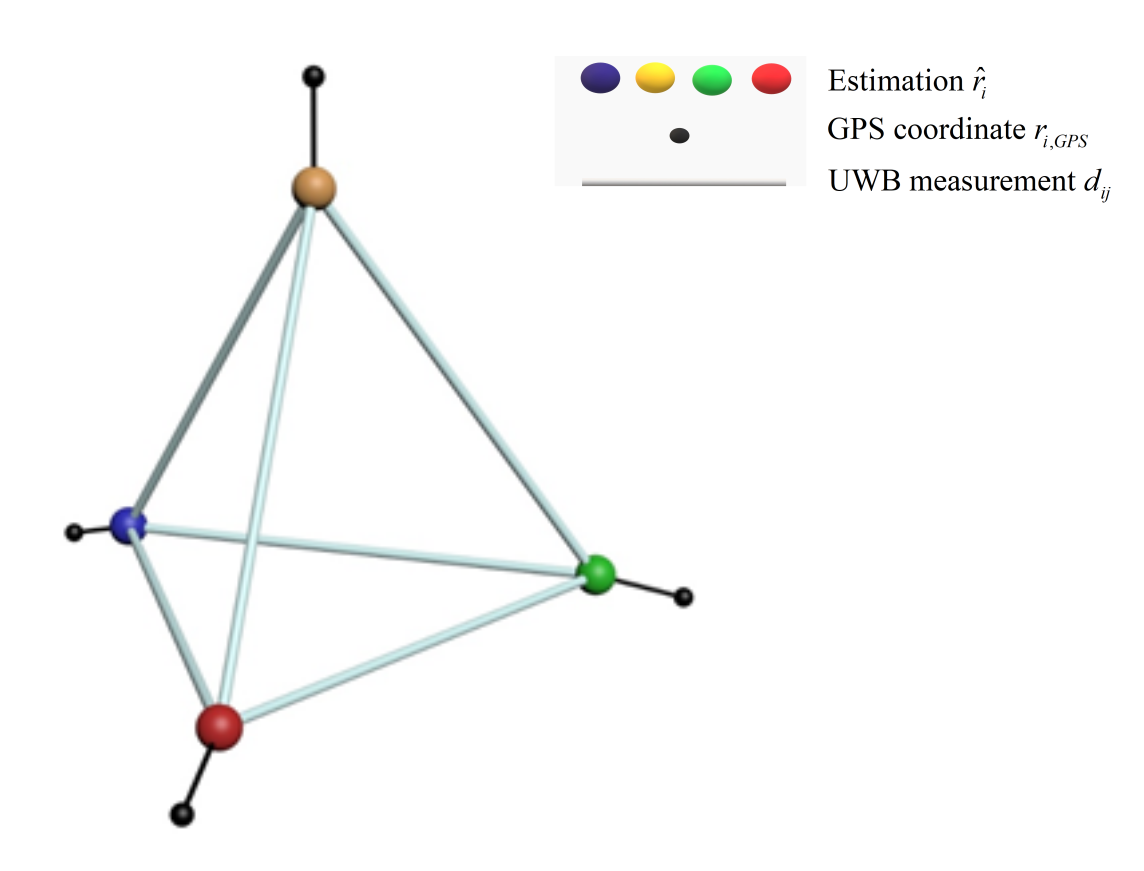
\includegraphics[width=0.5\linewidth]{Images/Related-Work/paper-spring.png}
	\decoRule
	\caption[An illustration of the spring system]{An illustration of the spring system based on \cite{uwb-imu-gps1} (\href{https://www.researchgate.net/publication/345459052_Cooperative_3-D_relative_localization_for_UAV_swarm_by_fusing_UWB_with_IMU_and_GPS}{URL})}
	\label{fig:spring-system}
\end{figure}

Σχετικά με το υλικό που χρησιμοποιήθηκε, έγινε χρήση ενός NEO-M8N \hyperref[abbr:GPS]{GPS} της U-blox με συχνότητα ανανέωσης τα 5Hz.  
Σε κάθε \hyperref[abbr:UAV]{UAV} χρησιμοποιήθηκε ένα Pixhawk PX4 flight management unit. Για το κομμάτι του \hyperref[abbr:UWB]{UWB} έγινε χρήση
ενός module LinkTrack, για την επικοινωνία με το ground station χρησιμοποιήθηκε ένα UBNT, ενώ τέλος η επεξεργασία των αλγορίθμων έγιναν 
σε ένα Raspberry Pi 3B+. 

Τέλος, τα αποτελέσματα που κατάφεραν να έχουν ήταν 3-D relative position estimation με σφάλμα απόκλισης τα 40cm. 

% ---------------------
\subsection{GSM/LTE/5G}
Ένας ακόμα εφικτός τρόπος προσέγγισης, για την εκτίμηση της θέσης είναι με χρήση
cellular networks.


% ---------------------
\subsection{RTK GNSS}
Ένας από τους τρόπους που μπορούν να χρησιμοποιηθούν προκειμένου να έχουμε ακρίβεια εκτίμησης
της θέσης των drone σε επίπεδο μερικών εκατοστών ($\sim$2-3cm)

% ------------------------------------------------------------------------------------
\section{Sound Waves}

\cite{sound-waves-for-drone-localization}

% ------------------------------------------------------------------------------------
\section{Image Oriented}

% ---------------------
\subsection{Motion Capturing System}

% ---------------------



